\documentclass[article]{jss}

%% -- LaTeX packages and custom commands ---------------------------------------

%% recommended packages
\usepackage{thumbpdf,lmodern}

%% additional packages
\usepackage{amssymb,amsmath}

%% new custom commands
\newcommand{\class}[1]{`\code{#1}'}
\newcommand{\fct}[1]{\code{#1()}}

%% For Sweave-based articles about R packages:
%% need no \usepackage{Sweave}



%% -- Article metainformation (author, title, ...) -----------------------------

%% - \author{} with primary affiliation
%% - \Plainauthor{} without affiliations
%% - Separate authors by \And or \AND (in \author) or by comma (in \Plainauthor).
%% - \AND starts a new line, \And does not.
\author{Lennart Oelschl\"ager \\Bielefeld University \And Dietmar Bauer\\Bielefeld University}
\Plainauthor{Lennart Oelschl\"ager, Dietmar Bauer}

%% - \title{} in title case
%% - \Plaintitle{} without LaTeX markup (if any)
%% - \Shorttitle{} with LaTeX markup (if any), used as running title
\title{\pkg{RprobitB}: Bayes Estimation of Discrete Choice Behavior Heterogeneity via Probit Models in \proglang{R}}
\Plaintitle{RprobitB: Bayes Estimation of Discrete Choice Behavior Heterogeneity via Probit Models in R}
\Shorttitle{RprobitB}

%% - \Abstract{} almost as usual
\Abstract{
\pkg{RprobitB} is an \proglang{R} package for Bayes estimation of probit models with a special focus on modeling choice behavior heterogeneity. In comparison to competing packages it places a focus on approximating the mixing distribution via a latent mixture of Gaussian distributions and thereby providing a classification of deciders. It provides tools for data management, model estimation via Markov Chain Monte Carlo Simulation, diagnostics tools for the Gibbs sampling and a prediction function. This paper demonstrates the functionalities of \pkg{RprobitB} on known choice datasets and compares estimation results across packages.
}

%% - \Keywords{} with LaTeX markup, at least one required
%% - \Plainkeywords{} without LaTeX markup (if necessary)
%% - Should be comma-separated and in sentence case.
\Keywords{discrete choice, probit models, heterogeneity, Bayes estimation, \proglang{R}}
\Plainkeywords{discrete choice, probit models, heterogeneity, Bayes estimation, R}

%% - \Address{} of at least one author
%% - May contain multiple affiliations for each author
%%   (in extra lines, separated by \emph{and}\\).
%% - May contain multiple authors for the same affiliation
%%   (in the same first line, separated by comma).
\Address{
  Lennart Oelschl\"ager, Dietmar Bauer\\
  Department of Business Administration and Economics\\
  Bielefeld University\\
  Postfach 10 01 31\\
  E-mail: \email{lennart.oelschlaeger@uni-bielefeld.de}, \email{dietmar.bauer@uni-bielefeld.de}
}

\begin{document}
%% I have no idea what this does. Maybe we need this in the future.
%% \SweaveOpts{concordance=TRUE}

%% -- Introduction -------------------------------------------------------------

%% - In principle "as usual".
%% - But should typically have some discussion of both _software_ and _methods_.
%% - Use \proglang{}, \pkg{}, \fct{} and \code{} markup throughout the manuscript.
%% - If such markup is in (sub)section titles, a plain text version has to be
%%   added as well.
%% - All software mentioned should be properly \cite-d.
%% - All abbreviations should be introduced.
%% - Unless the expansions of abbreviations are proper names (like "Journal
%%   of Statistical Software" above) they should be in sentence case (like
%%   "generalized linear models" below).

\section{Introduction}
\label{sec:introduction}

% Opening
Many applied research areas seek to understand decision maker's choices among a discrete set of alternatives, for example between different brands (marketing) or options to commute (transportation). Of central interest is heterogeneity in choice behavior: do deciders weight choice attributes like product price or travel time differently? If yes, to what extend? And what groups of deciders share similar preferences? Answering questions of this type is the motivation behind the presented statistical software \pkg{RprobitB} \citep{Oelschlaeger:2021}. The package name is a portmanteau of \proglang{R} (the programming language), the probit model class, and the Bayesian estimation framework.

% The mixed probit model
The probit model is one of the most widely-used statistical models to explain discrete choices.  Heterogeneity in choice behavior can be modeled using mixing distributions for the coefficients. Recently, \cite{Oelschlaeger:2020} proposed a new instrument for approximating the underlying mixing distribution that combines Bayes estimation and semi-parametric methods. This paper presents the implementation of the methodology in the \proglang{R} package \pkg{RprobitB}.

%% Overview RUMs
Traditionally, discrete choice models are interpreted as random utility models, including the multinomial logit (MNL) and the multinomial probit (MNP) model as the most prominent members. The MNL model affords straightforward analysis but suffers from the well-known independence of irrelevant alternatives assumption. In contrast, the MNP model avoids this assumption, which however comes at the price of more complex parameter estimation, cf.\ \cite{Train:2009}. In their basic form, these models often fail to take into account heterogeneity of individual deciders, cf.\ \cite{Train:2009}, Chapter 6, or \cite{Train:2016}. A concrete example of heterogeneous preferences is constituted by the value of travel time, cf.\ \cite{Cirillo:2006}. Modeling heterogeneity in preferences is indispensable in such cases and has been elaborated in both the MNL and the MNP model by imposing mixing distributions on the coefficients, cf.\ \cite{Train:2009} and \cite{Bhat:2011}.

% How are the mixing distribution specified currently?
Specifying these mixing distributions is an important part of the model selection. In absence of alternatives, it has been common practice so far to try different types of standard parametric distributions (including the normal, log-normal, uniform and tent distribution) and to perform a likelihood value-based model selection, cf.\ \cite{Train:2009}, Chapter 6. Aiming to capture correlation patterns across parameters, \cite{Fountas:2018} and \cite{Fountas:2019} apply multivariate normal mixing distributions in their probit models, which however comes at the price of imposing the rather strong normality assumption on their parameters.

In order to alleviate these restrictions \cite{Train:2016} proposes a non-parametric approach based on grid methods. Building on the ideas of \cite{Train:2016} and \cite{Bhat:2018} recently \cite{Bauer:2019} introduced procedures for non-parametrically estimating latent class mixed multinomial probit models where the number of classes is chosen iteratively in the algorithm. These procedures have been demonstrated to be useful in reasonable sized cross-sectional data sets. However, for large panel data sets with a significant number of choice occasions per person, the approach is numerically extremely demanding in particular due to its non-parametric nature and has to deal with the curse of dimensionality.

%What is the potential benefit of Bayesian estimation?
In the Bayesian framework \cite{Scaccia:2010} presents the idea to estimate latent class logit models with a fixed prespecified number of Gaussian components. This approach does not require the maximization of the likelihood while at the same time it allows for approximation of the underlying mixing distribution. The same idea has also been applied to probit models, cf.\ \cite{Xiong:2013} for an analysis of adolescent driver-injury data. In both cases however, the specification of the number of latent classes is based only on a trial-and-error strategy.

%What approach do we suggest to specify the mixing distributions?
Oelschlaeger and Bauer presents a more flexible approach that combines the ideas of a Bayesian framework, approximating the mixing distribution through a mixture of normal distributions and updates on the number of latent classes within the algorithm analogously to \cite{Bauer:2019}. As a consequence, the procedure unites the benefits of a reduced numerical complexity for the estimation compared to the non-parametric likelihood maximization approach and the ability to approximate any mixing distribution. Presenting simulation results on artificial test cases, it is shown that the approach is capable of approximating the underlying mixing distributions and thereby guiding the specification of mixing distributions for real-world applications.

% Comparison to other packages
This packages adds to the line of discrete choice software packages in R in the following way: Its focus is entirely on Bayesian estimation, thereby it differs from the packages Rchoice. Furthermore, it places a focus on modeling choice behaviour heterogeneity by approximating the underlying mixing distribution through a latent mixture of normal distributions. The method is explained in detail in Oelschlaeger and Bauer.

\begin{table}[!h]
\centering
\begin{tabular}{l|cccccccc}
               & Probit      & Logit      & Bayes      & ML         & Ord.       & Mix.       & LC           & upd. LC    \\ \hline
\pkg{Rchoice}  & \checkmark  & \checkmark &            & \checkmark & \checkmark & \checkmark &              &            \\
\pkg{mlogit}   & \checkmark  & \checkmark &            & \checkmark & \checkmark & \checkmark &              &            \\
\pkg{Biogeme}  & \checkmark  & \checkmark &            & \checkmark & \checkmark & \checkmark & \checkmark   &            \\
\pkg{apollo}   & \checkmark  & \checkmark & \checkmark & \checkmark & \checkmark & \checkmark & \checkmark   &            \\
\pkg{bayesm}   & \checkmark  & \checkmark & \checkmark &            & \checkmark & \checkmark &              &            \\
\pkg{MNP}      & \checkmark  &            & \checkmark &            & \checkmark &            &              &            \\
\pkg{RprobitB} & \checkmark  &            & \checkmark &            &            & \checkmark & \checkmark   & \checkmark \\
\end{tabular}
\label{tab:pkg_overview}
\caption{Overview of packages for discrete choice modeling.}
\end{table}

% Examples
\begin{table}[!h]
\centering
\begin{tabular}{l|p{10cm}}
Example                     & Illustrated package functionalities \\ \hline
1: Train                    & \fct{prepare\_data}, \fct{fit\_model}, \fct{predict}, \fct{model\_selection} \\
2: Simulated choices        & \fct{simulate\_choices}, estimation and weight-based update of latent classes \\
3: Electricity              & estimation and interpretation of random effects \\
4: Online chess strategy    & Dirichlet process-based update of latent classes, preference classification \\
\end{tabular}
\label{tab:example_overview}
\caption{Overview of examples.}
\end{table}

%% Article overview
In this article we present the methodology, give an overview over the functionality of the package and apply the package to data sets. Some of them were already analysed and we aim to reconstruct their findings. In addition, we added two datasets that are especially appropriate for \pkg{RprobitB} in modeling choice behaviour heterogeneits. The first one is a dataset of contraception choice from the German family panel pairfam. It contains repeated observations of males and femals over several years having different social demographics and relationship status choosing different means of contraception. This choice a priori can be considered to be very hetereogenous and dependent on factors not directly observable by the researcher. The second application deals with the opening choice of chess players depending on their and their openents playing strenght measured in the popular measure system Elo, their gender and nationality. Like the contraception example, this choice a priori can be considers to depend on psychological factors that are not directly observable by the researcher. By applying the functionality of this package we demonstrate how we are able to classify the players into different categories of playing style.

% Dirichlet process
A similar approach in the context of discrete choice can be found in \cite{Burda:2008}, where the Dirichlet process is applied to estimate a mixed logit-probit model.

1. With \pkg{RprobitB}, you can model the choices made by deciders among a discrete set of alternatives. For example, think of tourists that want to book a flight to their holiday destination. The knowledge why they prefer a certain route over another is of great value for airlines, especially the customer's willingness to pay for say a faster or more comfortable flight alternative.

2. Different deciders value different choice attributes differently. For example, it is imaginable that business people place a higher value on flight time and are willing to pay more for a faster route alternative than vacationers. Such choice behavior heterogeneity can be addressed by \pkg{RprobitB}. Furthermore, the package enables to identify groups of deciders that share similar preferences.

3. Finally, the package enables prediction of choice behavior when certain choice attributes change, for example the proportion of customers who will choose the competitor's product in the event of a price increase.

The functions of \pkg{RprobitB} can be grouped into ones for data management, model fitting, and model evaluation, see the flowchart below. The package can be used for two different purposes: (a) estimation of a model for given data and (b) estimation of a model for simulated data. Simulation typically serves to assess the properties of estimation algorithms either for research or in a bootstrap like fashion. \pkg{RprobitB} supports these functions.

\begin{figure}[t!]
  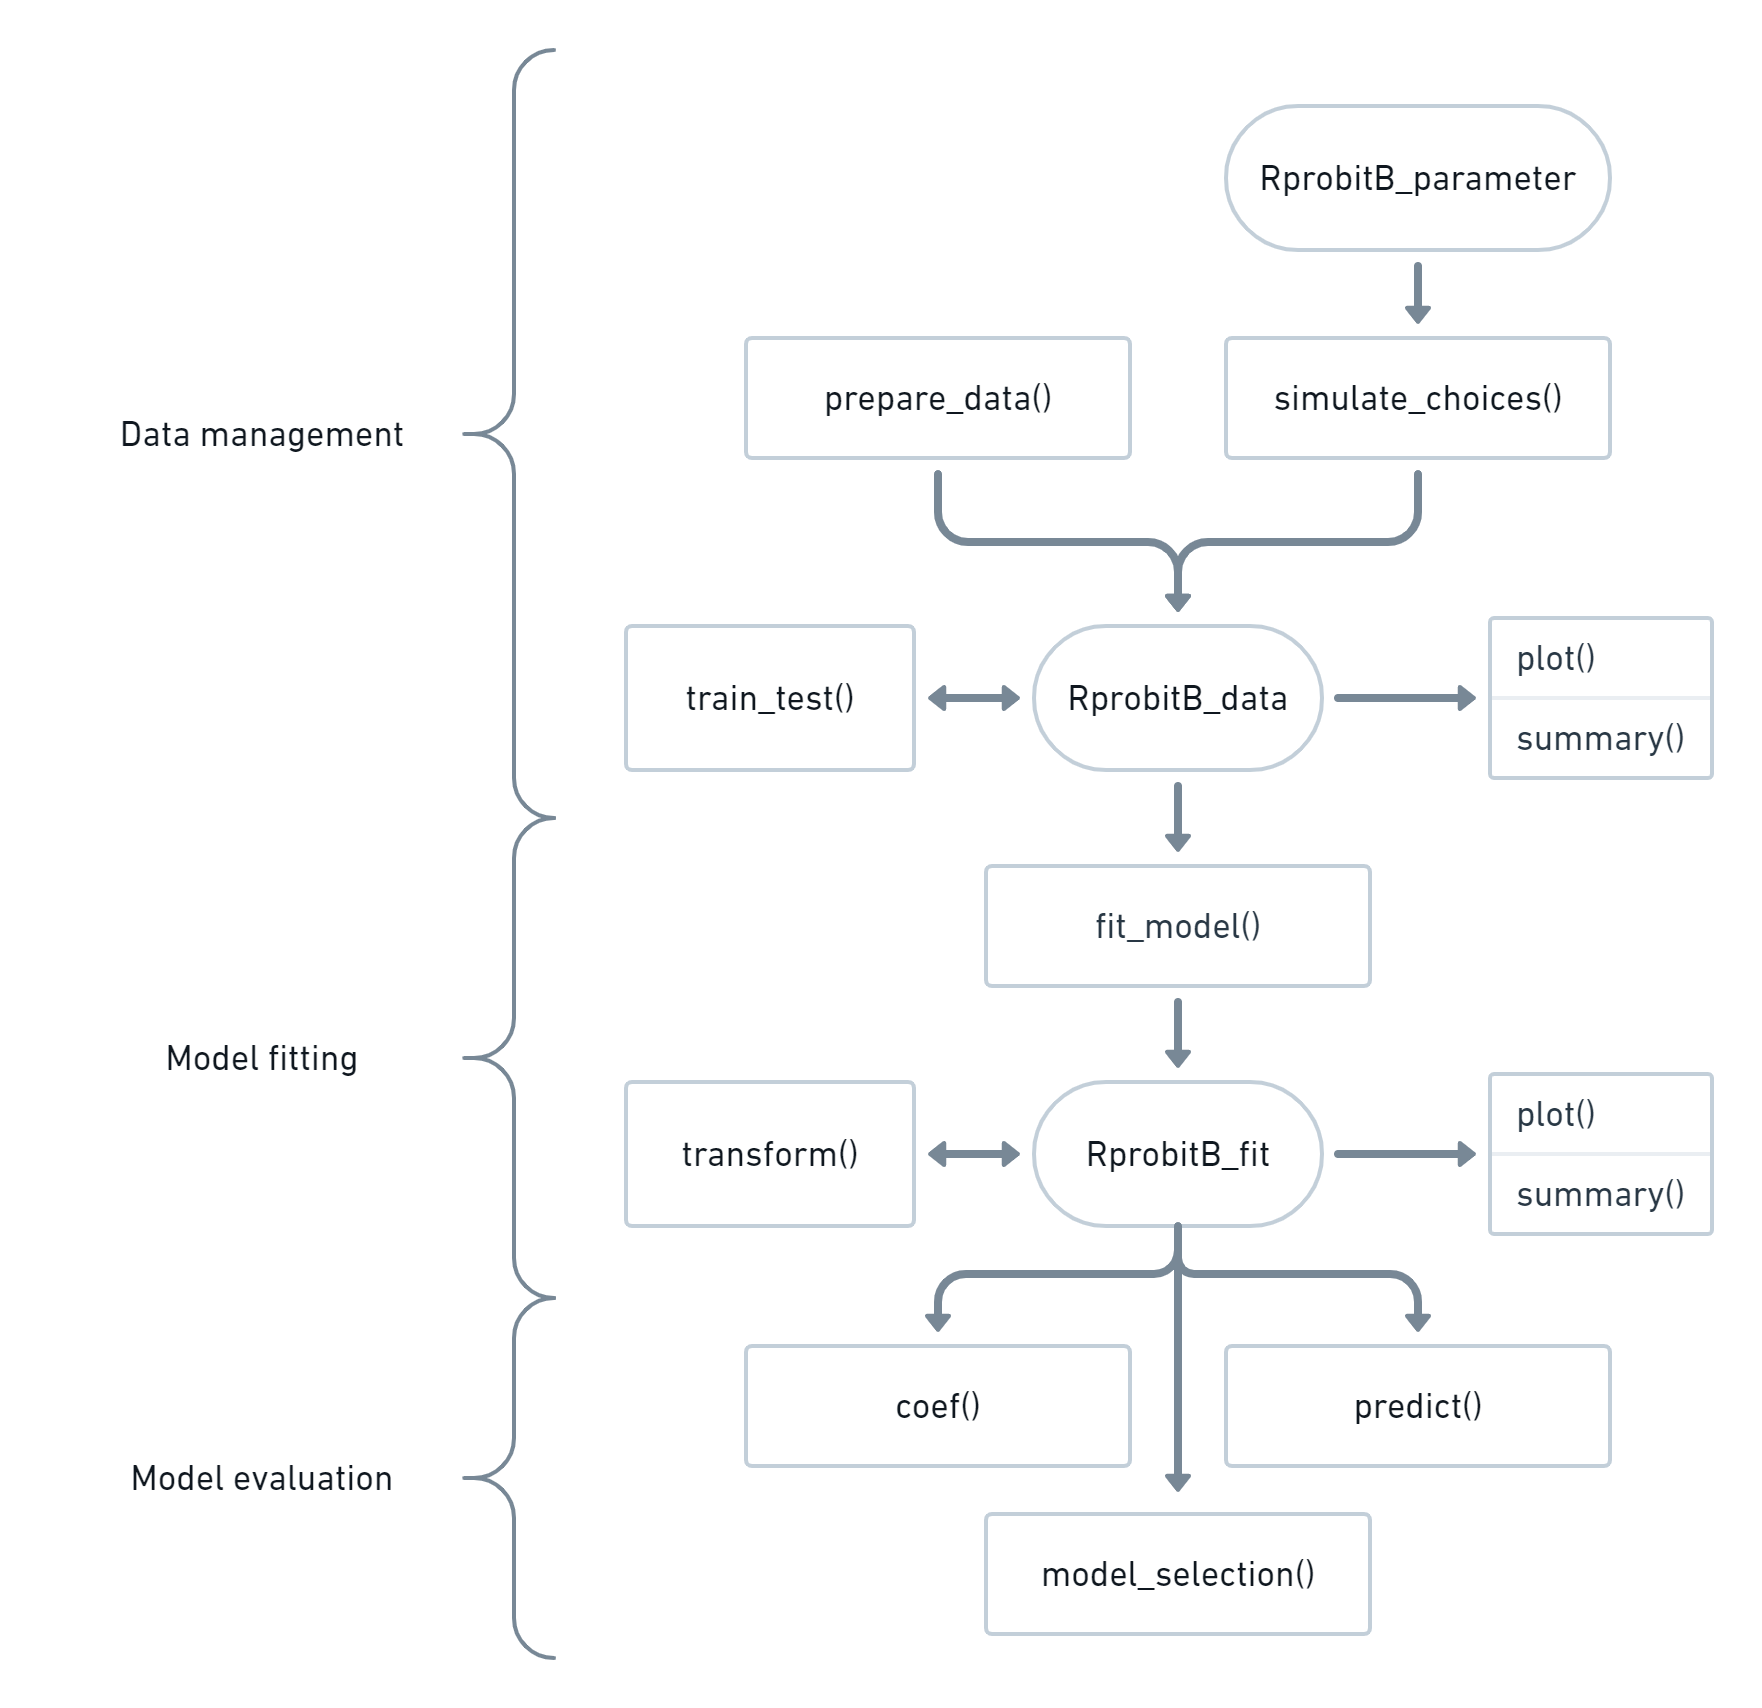
\includegraphics{flowchart.png}
  \caption{Package flowchart with main functions as rectangles and objects as ovals.}
  \label{fig:flowchart}
\end{figure}


\section{The probit model} \label{sec:probit_model}

To fix our notation, this section briefly defines the probit model based on the concept of latent utilities, introduces mixing distributions for addressing choice behavior heterogeneity, and discusses required model normalization for parameter identification.

\subsection{Latent utilities} \label{subsec:latent_utilities}

Assume that we know the choices of $N$ deciders choosing between $J \geq 2$ alternatives at each of $T$ choice occasions.\footnote{The number $T$ of choice occasions is the same for each decider here for notational simplicity. However, \pkg{RprobitB} allows for unbalanced panels, i.e.\ varying $T$. Of course, the cross-sectional case $T = 1$ is possible.} Specific to each decider, alternative and choice occasion, we observe $P$ covariates. We seek to explain the choices by a linear combination of those:
\begin{equation}
  \label{eq:utility}
  U_{ntj} = X_{ntj}'\beta + \epsilon_{ntj}
\end{equation}
for $n=1,\dots,N$, $t=1,\dots,T$ and $j=1,\dots,J$. Here, $X_{ntj}$ is a (column) vector of $P$ characteristics of alternative $j$ as faced by decider $n$ at choice occasion $t$, $\beta \in {\mathbb R}^{P}$ is a vector of coefficients, and $(\epsilon_{nt:}) = (\epsilon_{nt1},\dots,\epsilon_{ntJ})' \sim \text{MVN}_{J} (0,\Sigma)$ is the model's error term vector for $n$ at $t$.\footnote{The assumption that the error terms are multivariate normally distributed distinguishes the probit from the logit model: in the latter, each $\epsilon_{ntj}$ is assumed to be independently extreme value distributed.} The values $U_{ntj}$ are latent and can be interpreted as $n$'s utility of $j$ at $t$. We assume utility maximizing behavior of the deciders\footnote{We note that utility maximizing behavior is a common assumption in econometric models. However, many studies have shown that humans do not decide in this rational sense in general, see for example \cite{Hewig:2011}.} and link the latent utilities to the choices via
\begin{align*}
   y_{nt} = \operatorname*{argmax}_{j = 1,\dots,J} U_{ntj},
\end{align*}
where $y_{nt}=j$ denotes the event that decider $n$ chooses $j$ at $t$.

\subsection{Choice behavior heterogeneity} \label{subsec:heterogeneity}

The coefficient vector $\beta$ in equation \eqref{eq:utility} is constant across decision makers. This assumption is too restrictive for many applications\footnote{As an example, consider the choice of a means of transportation: it is easily imaginable that business people and pensioners do not share the same sensitivities towards cost and time. \cite{Cirillo:2006} identifies such heterogeneity in an empirical study on the basis of travel diaries.} and can be relaxed by imposing a distribution on $\beta$ \citep[Ch.\ 6]{Train:2009}. Then, each decider $n$ can have their own sensitivities $\beta_n$ as a realization from this underlying mixing distribution. In \pkg{RprobitB}, we allow for a combination of such random effects next to fixed effects by replacing $\beta$ in equation \eqref{eq:utility} with $\beta = (\alpha, \beta_n)$, where $\alpha$ are $P_f$ coefficients that are constant across deciders and $\beta_n$ are $P_r$ decider specific coefficients, $P_f + P_r = P$. Now if $P_r>0$, $\beta_n$ is distributed according to some $P_r$-variate mixing distribution.

Choosing an appropriate mixing distribution is a notoriously difficult task of the model specification. In many applications, different types of standard parametric distributions (including the normal, log-normal, uniform and tent distribution) are tried in conjunction with a likelihood value-based model selection \citep[pp.\ 136 ff.\ ]{Train:2009}. Instead, \pkg{RprobitB} implements the approach of \cite{Oelschlaeger:2020} to approximate any underlying mixing distribution by a mixture of $P_r$-variate Gaussian densities $\phi_{P_r}$ with mean vectors $b=(b_c)_{c}$ and covariance matrices $\Omega=(\Omega_c)_{c}$ using $C$ components:
\begin{align*}
\beta_n\mid b,\Omega \sim \sum_{c=1}^{C} s_c \phi_{P_r} (\cdot \mid b_c,\Omega_c).
\end{align*}
Here, $(s_c)_{c}$ are weights satisfying $0 < s_c\leq 1$ for $c=1,\dots,C$ and $\sum_c s_c=1$. One interpretation of the latent class model is obtained by introducing variables $z=(z_n)_n$, allocating each decision maker $n$ to class $c$ with probability $s_c$, i.e.\
\begin{align*}
\text{Prob}(z_n=c)=s_c \land \beta_n \mid z,b,\Omega \sim \phi_{P_r}(\cdot \mid b_{z_n},\Omega_{z_n}).
\end{align*}
This interpretation allows for preference classifications, see Section \ref{subsec:dp_update} for an example.

\subsection{Model normalization} \label{subsec:normalization}

Any utility model is invariant towards the level and the scale of utility \citep[Ch.\ 2]{Train:2009}. For identification of the model parameters, we therefore normalize the model by taking utility differences and fixing one error term variance. Formally, equation \eqref{eq:utility} is transformed to
\begin{align*}
\tilde{U}_{ntj} = \tilde{X}_{ntj}' \beta + \tilde{\epsilon}_{ntj},
\end{align*}
$j=1,\dots,J-1$, where (choosing $J$ as the reference alternative), $\tilde{U}_{ntj} = U_{ntj} - U_{ntJ}$, $\tilde{X}_{ntj} = X_{ntj} - X_{ntJ}$, and $\tilde{\epsilon}_{ntj} = \epsilon_{ntj} - \epsilon_{ntJ}$. The error term differences $(\tilde{\epsilon}_{nt:}) = (\tilde{\epsilon}_{nt1},...,\tilde{\epsilon}_{nt(J-1)})'$ again are multivariate normally distributed with mean 0 but transformed covariance matrix $\tilde{\Sigma}$, in which one diagonal element is fixed to a positive number.\footnote{Fixing one element of $\tilde{\Sigma}$ determines the utility scale. Fixing one fixed effect (i.e.\ one entry of $\alpha$) serves the same purpose. Both alternatives are implemented in \pkg{RprobitB}, see Section \ref{subsec:estimation_routine}.}

\section{Choice data} \label{sec:choice_data}

\pkg{RprobitB} requests that choice data sets are (a) of class \class{data.frame} and (b) in wide format (that means each row provides the full information for one choice occasion), (c) contain a column with unique identifiers for each decision maker (and optionally each choice occasion), (d) contain a column with the observed choices (required for model fitting but not for prediction), and (e) contain columns for the values of alternative and/or decider specific covariates. The underlying set of choice alternatives is assumed to be mutually exclusive (one can choose one and only one alternative that are all different), exhaustive (the alternatives do not leave other options open), and finite \citep[Ch.\ 2]{Train:2009}.

This section introduces the package's formula framework for specifying the set of covariates entering a model. The framework is adapted from \pkg{mlogit}, which is flexible enough to allow for different types of covariates: covariates that are constant across alternatives (e.g.\ the decider's age), covariates that are alternative specific (e.g.\ the alternative's price), covariates with a generic coefficient (e.g.\ paying the same amount of money for train company A versus B should make no difference), and covariates that have alternative specific coefficients (e.g.\ spending time in a crowded train versus a private jet makes a difference). Subsequently, we demonstrate how to pass such a formula to the functions \fct{prepare\_data} for preparing empirical data for estimation and \fct{simulate\_choices} for simulating choice data.

\subsection{Formula framework} \label{subsec:formula}

We generalize equation \eqref{eq:utility} to allow for different types of covariates:
\begin{align}
  \label{eq:utility_gen}
  U_{ntj} = A_{ntj} \beta_1 + B_{nt} \beta_{2j} + C_{ntj} \beta_{3j} + \epsilon_{ntj},
\end{align}
where the covariates $A$ and $C$ depend on the alternative and $B$ is only choice occasion specific. The coefficient $\beta_1$ is generic (i.e.\ the same for each alternative), whereas $\beta_{2j}$ and $\beta_{3j}$ are alternative specific. Note that the full collection $(\beta_{2j})_{j=1,\dots,J}$ is not identified: because we took utility differences for model normalization (cf.\ Section \ref{subsec:normalization}), one coefficient is a linear combination of the others. We therefore fix $\beta_{2k}$ to 0 for one base alternative $k$. The coefficients $(\beta_{2j})_{j\neq k}$ then have to be interpreted with respect to the base alternative.

Equation \eqref{eq:utility_gen} can be entered into \proglang{R} via specifying the \class{formula} object \code{choice ~ A | B | C}, where \code{choice} is the name of the dependent variable (the discrete choice we aim to explain). By default, alternative specific constants (ASCs)\footnote{ASCs capture the average effect on utility of all factors that are not included in the model. We cannot estimate ASCs for all the alternatives due to identifiability. Therefore, they are added for all except for the base alternative.} are added to the model. They can be removed by adding \code{+ 0} in the second spot, e.g.\ \code{choice ~ A | B + 0 | C}. To exclude covariates of the backmost categories, use either \code{0}, e.g.\ \code{choice ~ A | B | 0} or just leave this part out and write \code{choice ~ A | B}. However, to exclude covariates of front categories, we have to use \code{0}, e.g.\ \code{choice ~ 0 | B}. To include more than one covariate of the same category, use \code{+}, e.g.\ \code{choice ~ A1 + A2 | B}. If we don't want to include any covariates of the second category but want to estimate ASCs, add \code{1} in the second spot, e.g.\ \code{choice ~ A | 1 | C}. The expression \code{choice ~ A | 0 | C} is interpreted as no covariates of the second category and no alternative specific constants.

\subsection{Preparing data for estimation} \label{subsec:prepare_data}

Before model estimation, any choice data set \code{choice\_data} must pass the \fct{prepare\_data} function together with a formula object \code{form} introduced above:

\begin{Schunk}
\begin{Sinput}
> data <- prepare_data(form = form, choice_data = choice_data)
\end{Sinput}
\end{Schunk}

The function performs compatibility checks and data transformations and returns an object of class \class{RprobitB\_data} that can be fed into the estimation routine \fct{fit\_model} (introduced in Section \ref{sec:model_fitting}). The following arguments of \fct{prepare\_data} are optional:
\begin{itemize}
  \item \code{re}: A character vector of covariate names in \code{form} with random effects (cf.\ Section \ref{subsec:heterogeneity}). Per default \code{re = NULL}, i.e.\ no random effects.
  \item \code{alternatives}: A character vector of alternative names, defining the choice set. If not specified, all alternatives chosen in the data set are considered.
  \item \code{base}: One element of \code{alternatives} specifying the base alternative (cf.\ Section \ref{subsec:formula}). Per default, \code{base} is the last element of \code{alternatives}.
  \item \code{id} and \code{idc}: The names of the columns in \code{choice_data} that contain unique identifier for each decision maker and for each choice occasion, respectively. Per default, \code{id = "id"} and \code{idc = NULL}, in which case the choice occasion identifier are generated by the appearance of the choices in the data set.
  \item \code{standardize}: A character vector of variable names of \code{form} that get standardized, i.e.\ rescaled to have a mean of 0 and a standard deviation of 1 (none per default).
  \item \code{impute}: A character, specifying how to handle missing data entries. Options are \code{"complete\_cases"} (removing rows that contain missing entries, which is the default behavior), \code{"zero"} (replacing missing entries by 0), and \code{"mean"} (imputing missing entries by the covariate mean).
\end{itemize}

\paragraph{Example 1: Train trips.}

The \pkg{mlogit} package provides the data set \code{Train}, which contains 2929 stated choices of 235 deciders between two fictional train trip alternatives \code{A} and \code{B}. The trip alternatives are characterized by their \code{price}, the travel \code{time}, the level of \code{comfort} (the lower the value the higher the comfort), and the number of \code{change}s. The data is in wide format; the columns \code{id} and \code{choiceid} identify the deciders and the choice occasions, respectively; the column \code{choice} provides the choices. For convenience, we transform \code{time} from minutes to hours and \code{price} from guilders to euros:

\begin{Schunk}
\begin{Sinput}
> data("Train", package = "mlogit")
> Train$price_A <- Train$price_A / 100 * 2.20371
> Train$price_B <- Train$price_B / 100 * 2.20371
> Train$time_A <- Train$time_A / 60
> Train$time_B <- Train$time_B / 60
> str(Train)
\end{Sinput}
\begin{Soutput}
'data.frame':	2929 obs. of  11 variables:
 $ id       : int  1 1 1 1 1 1 1 1 1 1 ...
 $ choiceid : int  1 2 3 4 5 6 7 8 9 10 ...
 $ choice   : Factor w/ 2 levels "A","B": 1 1 1 2 2 2 2 2 1 1 ...
 $ price_A  : num  52.9 52.9 52.9 88.1 52.9 ...
 $ time_A   : num  2.5 2.5 1.92 2.17 2.5 ...
 $ change_A : num  0 0 0 0 0 0 0 0 0 0 ...
 $ comfort_A: num  1 1 1 1 1 0 1 1 0 1 ...
 $ price_B  : num  88.1 70.5 88.1 70.5 70.5 ...
 $ time_B   : num  2.5 2.17 1.92 2.5 2.5 ...
 $ change_B : num  0 0 0 0 0 0 0 0 0 0 ...
 $ comfort_B: num  1 1 0 0 0 0 1 0 1 0 ...
\end{Soutput}
\end{Schunk}

For demonstration, say we want to include all choice characteristics into our probit model, connect them to generic coefficients, and exclude ASCs. We would specify the formula:

\begin{Schunk}
\begin{Sinput}
> form <- choice ~ price + time + comfort + change | 0
\end{Sinput}
\end{Schunk}

Passing \code{form} to \fct{prepare\_data} returns an \class{RprobitB\_data} object, which in turn can be fed into the estimation routine \fct{fit\_model} (cf.\ Section \ref{sec:model_fitting}):

\begin{Schunk}
\begin{Sinput}
> data_train <- prepare_data(
+    form = form, choice_data = Train, id = "id", idc = "choiceid"
+  )
\end{Sinput}
\end{Schunk}

The data object can be inspected via its \fct{summary} and \fct{plot} methods:

\begin{Schunk}
\begin{Sinput}
> summary(data_train)
\end{Sinput}
\begin{Soutput}
  number deciders choice occasions choices total
1             235     5 to 19 each          2929

  alternative frequency
1           A      1474
2           B      1455
\end{Soutput}
\end{Schunk}

\begin{Schunk}
\begin{Sinput}
> plot(data_train)
\end{Sinput}
\end{Schunk}
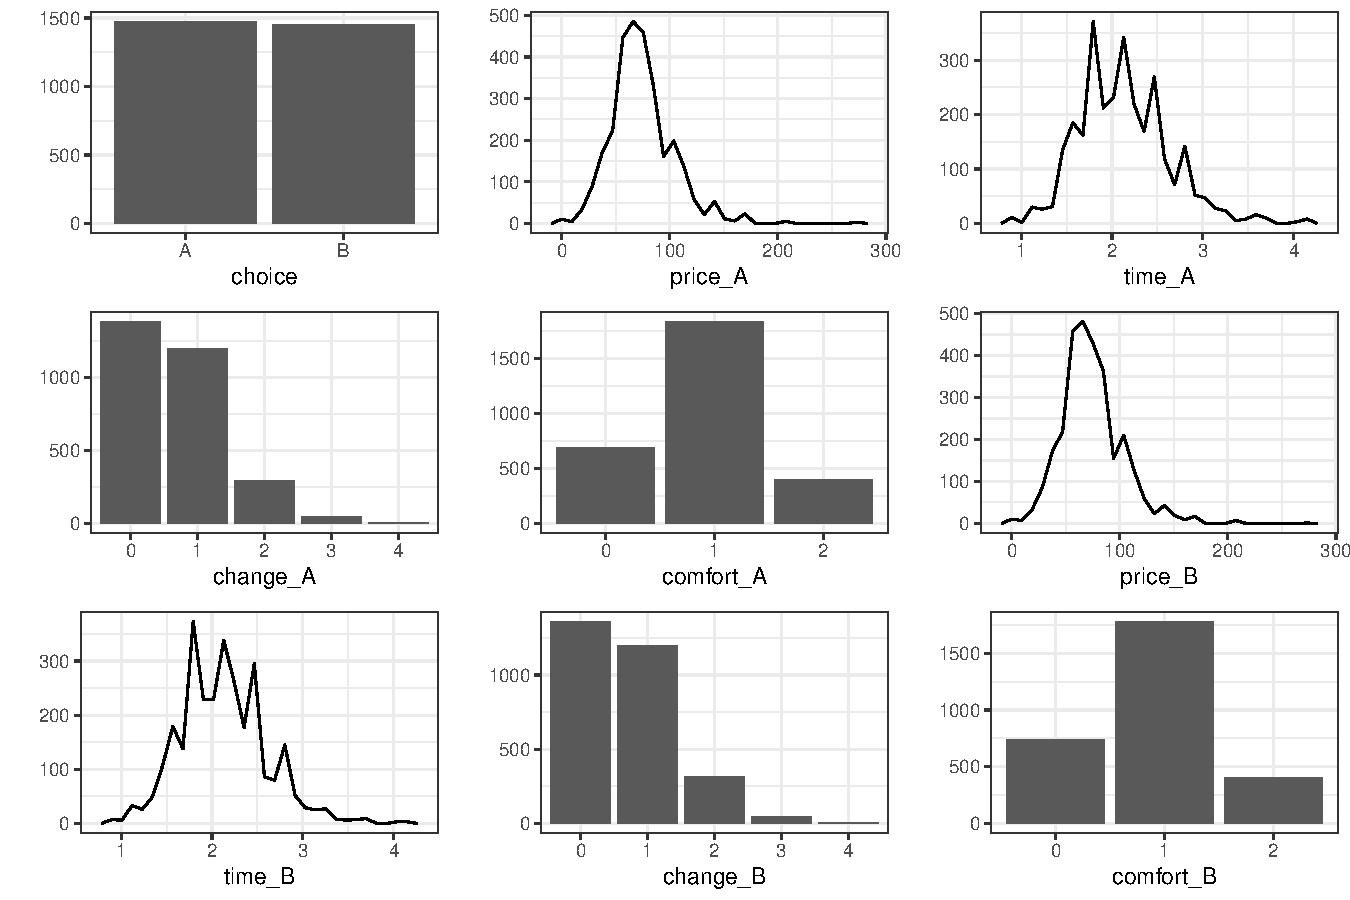
\includegraphics{rprobitb_oelschlaeger_bauer-train-data}

\subsection{Simulating choice data} \label{subsec:simulate_choice_data}

The \fct{simulate\_choices} function simulates choice data from a pre-specified probit model. Say we want to simulate the choices of \code{N} deciders in \code{T} choice occasions\footnote{\code{T} can be either a positive number, representing a fixed number of choice occasions for each decision maker, or a vector of length \code{N} with decision maker specific numbers of choice occasions} among \code{J} alternatives. Together with a model formula \code{form}, we would have to call

\begin{Schunk}
\begin{Sinput}
> data <- simulate_choices(form = form, N = N, T = T, J = J)
\end{Sinput}
\end{Schunk}

The function \fct{simulate\_choices} has the following optional arguments:
\begin{itemize}
  \item \code{re}, \code{base}, \code{standardize}: Analogue to \fct{prepare\_data} (cf.\ Section \ref{subsec:prepare_data}).
  \item \code{alternatives}: A character vector of length \code{J} with the names of the choice alternatives (per default the first \code{J} upper-case letters of the Roman alphabet).
  \item \code{covariates}: A named list of covariate values. Each element must be a vector of length equal to the number of choice occasions and named according to a covariate. Unspecified covariates are drawn from a standard normal distribution.
  \item \code{seed}: Optionally set a seed for the simulation.
\end{itemize}

The true model parameters are set at random per default. Alternatively, they can be specified via a named list that is passed to the function's \code{true\_parameter} argument and contains:
\begin{itemize}
  \item a numeric vector \code{alpha} with the fixed effects,
  \item the number \code{C} of latent classes (\code{C = 1} per default),
  \item a numeric vector \code{s} of length \code{C} with the class weights,
  \item a matrix \code{b} with the class means as columns,
  \item a matrix \code{Omega} with the class covariance matrices as columns,
  \item a matrix \code{Sigma\_full} (\code{Sigma}), the (differenced) error term covariance matrix,
  \item a matrix \code{beta} with the decision-maker specific coefficient vectors as columns,
  \item a numeric vector \code{z} of length \code{N} with elements in \code{1:C}, representing the class allocations.
\end{itemize}

\paragraph{Example 2: Simulated choices.} For illustration, we simulate the choices of \code{N = 100} deciders at \code{T = 30} choice occasions between the fictitious alternatives \code{alt1} and \code{alt2}. The choices are explained by the alternative specific covariates \code{var1} and \code{var3}. Covariate \code{var2} is only choice occasion specific but connected to a random effect, as well as the ASCs:

\begin{Schunk}
\begin{Sinput}
> N <- 100
> T <- 30
> alternatives <- c("alt1", "alt2")
> form <- choice ~ var1 | var2 | var3
> re <- c("ASC","var2")
\end{Sinput}
\end{Schunk}

The \fct{overview\_effects} function provides an overview of the effect types:

\begin{Schunk}
\begin{Sinput}
> overview_effects(form = form, re = re, alternatives = alternatives)
\end{Sinput}
\begin{Soutput}
     effect as_value as_coef random
1      var1     TRUE   FALSE  FALSE
2 var3_alt1     TRUE    TRUE  FALSE
3 var3_alt2     TRUE    TRUE  FALSE
4 var2_alt1    FALSE    TRUE   TRUE
5  ASC_alt1    FALSE    TRUE   TRUE
\end{Soutput}
\end{Schunk}

The model has three fixed effects (\code{random = FALSE}), consequently the vector \code{alpha} must be of length 3, where the elements 1 to 3 correspond to \code{var1}, \code{var3\_alt1}, and \code{var3\_alt2}, respectively. Additionally, the model has two random effects (\code{random = TRUE}), hence the matrix \code{b} must be of dimension \code{2 x C}, where row 1 and 2 correspond to \code{var2\_alt1} and \code{ASC\_alt1}, respectively. We specify \code{C = 2} latent classes in the data generating process, which we will reproduce in Sections \ref{subsec:latent_classes} and \ref{subsec:weight_update}:

\begin{Schunk}
\begin{Sinput}
> data_sim <- simulate_choices(
+    form = form, N = N, T = T, J = 2,
+    re = re, alternatives = alternatives, seed = 1,
+    true_parameter = list(alpha = c(-1,0,1), C = 2, s = c(0.7,0.3),
+                          b = matrix(c(2,-0.5,1,1), ncol = 2), Sigma = 1)
+  )
\end{Sinput}
\end{Schunk}

The \fct{plot} method of \class{RprobitB\_data} objects has the optional argument \code{by\_choice}. Setting \code{by\_choice = TRUE} visualizes the (randomly drawn) covariates grouped by the chosen alternatives:

\begin{Schunk}
\begin{Sinput}
> plot(data_sim, by_choice = TRUE)
\end{Sinput}
\end{Schunk}
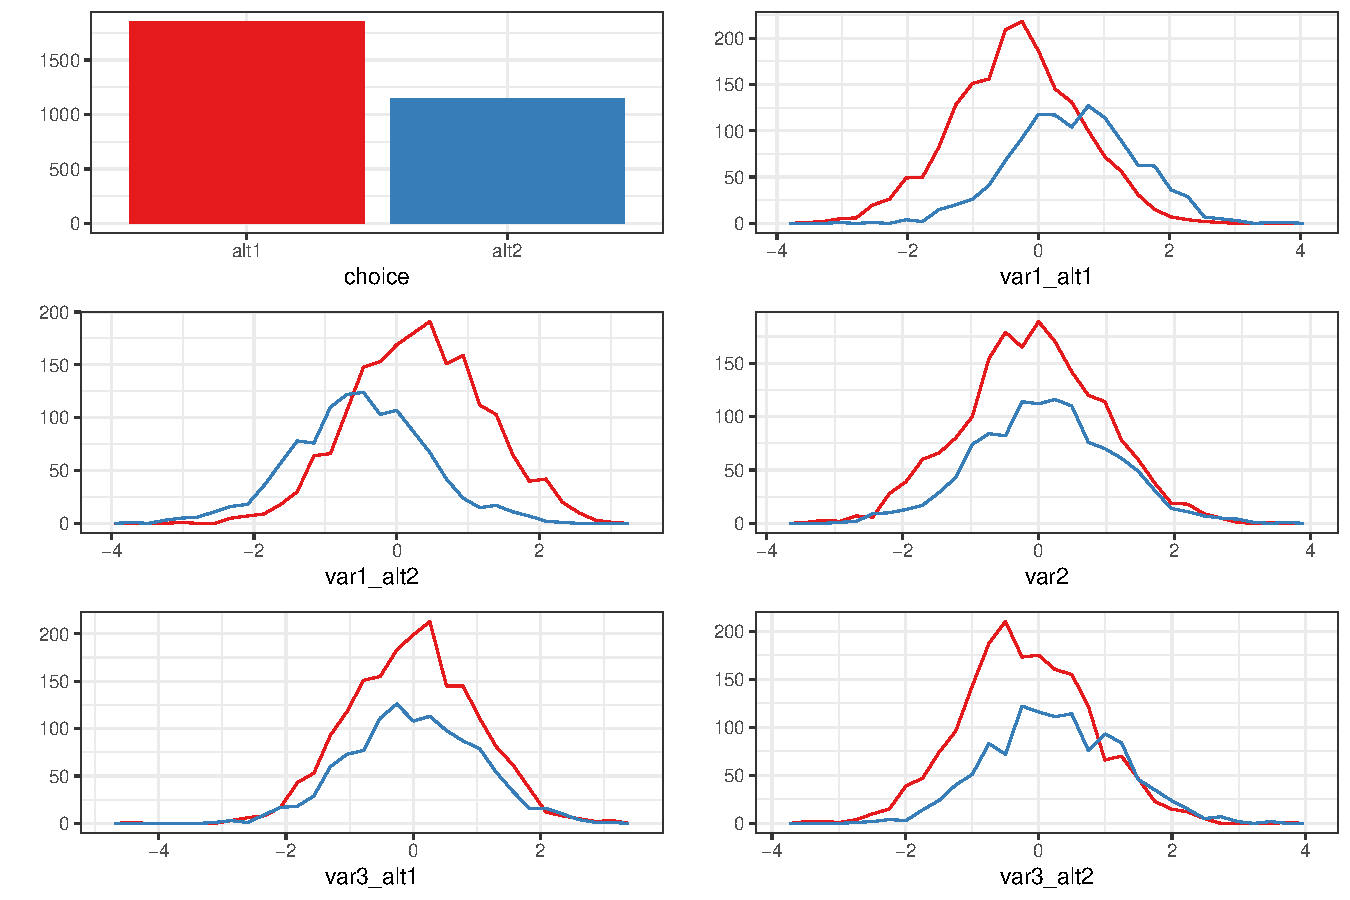
\includegraphics{rprobitb_oelschlaeger_bauer-sim-data}

The graphic is consistent with our model specification: for example, covariate \code{var1} was specified to have a negative effect on \code{alt1}, because the coefficient of \code{var1} (the first value of \code{alpha}) is negative $(-1)$. Hence, higher values of \code{var1\_alt1} correspond more frequently to choice \code{alt2} (upper-right panel).

\section{Model fitting} \label{sec:model_fitting}

\pkg{RprobitB} estimates the probit model in a Bayesian framework that builds upon the work of \cite{McCulloch:1994}, \cite{Nobile:1998}, \cite{Allenby:1998}, and \cite{Imai:2005}. A key ingredient is the concept of data augmentation \citep{Albert:1993}, which treats the latent utilities in model equation \eqref{eq:utility} as additional parameters. Then, conditional on these parameters, the probit model constitutes a standard Bayesian linear regression set-up. Its posterior distribution can be approximated via Gibbs sampling.

In the following, we list the prior distributions for the model parameters, formulate the conditional posterior distributions, introduce the estimation routine \fct{fit\_model}, and apply it to the two examples from the previous section. The remainder of this section is devoted to the estimation of latent class models and the implemented class updating schemes.

\subsection{Prior and posterior distributions} \label{subsec:prior_and_posterior}

We a priori assume the following (conjugate) parameter distributions:
\begin{itemize}
  \item $(s_1,\dots,s_C)\sim D_C(\delta)$, where $D_C(\delta)$ denotes the $C$-dimensional Dirichlet distribution with concentration parameter vector $\delta = (\delta_1,\dots,\delta_C)$,
  \item $\alpha\sim \text{MVN}_{P_f}(\psi,\Psi)$, where $\text{MVN}_{P_f}$ denotes the $P_f$-dimensional normal distribution with mean $\psi$ and covariance $\Psi$,
  \item $b_c \sim \text{MVN}_{P_r}(\xi,\Xi)$, independent for all $c$,
  \item $\Omega_c \sim W^{-1}_{P_r}(\nu,\Theta)$, independent for all $c$, where $W^{-1}_{P_r}(\nu,\Theta)$ denotes the $P_r$-dimensional inverse Wishart distribution with $\nu$ degrees of freedom and scale matrix $\Theta$,
  \item and $\tilde{\Sigma} \sim W^{-1}_{J-1}(\kappa,\Lambda)$.
\end{itemize}

These priors imply the following conditional posterior distributions (we are closely following \cite{Oelschlaeger:2020}):
\begin{itemize}
  \item The class weights are drawn from the Dirichlet distribution
  \begin{align*}
  (s_1,\dots,s_C)\mid \delta,z \sim D_C(\delta_1+m_1,\dots,\delta_C+m_C),
  \end{align*}
  where $m_c=\#\{n:z_n=c\}$ denotes the current absolute size of class $c$. The model is invariant to permutations of the class labels $1,\dots,C$. We therefore accept an update only if the ordering $s_1>\dots>s_C$ still holds (thereby ensuring a unique class labeling).
  \item The allocation variables $(z_n)_n$ are updated independently for all $n$ via
  \begin{align*}
  \text{Prob}(z_n=c\mid s,\beta,b,\Omega )=\frac{s_c\phi_{P_r}(\beta_n\mid b_c,\Omega_c)}{\sum_c s_c\phi_{P_r}(\beta_n\mid b_c,\Omega_c)}.
  \end{align*}
  \item The class means $(b_c)_c$ are updated independently for all $c$ via
  \begin{align*}
  b_c\mid \Xi,\Omega,\xi,z,\beta \sim\text{MVN}_{P_r}\left( \mu_{b_c}, \Sigma_{b_c}  \right),
  \end{align*}
  $\mu_{b_c}=(\Xi^{-1}+m_c\Omega_c^{-1})^{-1}(\Xi^{-1}\xi +m_c\Omega_c^{-1}\bar{b}_c)$, $\Sigma_{b_c}=(\Xi^{-1}+m_c\Omega_c^{-1})^{-1}$, $\bar{b}_c=m_c^{-1}\sum_{n:z_n=c} \beta_n$.
    \item The class covariance matrices $(\Omega_c)_c$ are updated independently for all $c$ via
  \begin{align*}
  \Omega_c \mid \nu,\Theta,z,\beta,b \sim W^{-1}_{P_r}(\mu_{\Omega_c},\Sigma_{\Omega_c}),
  \end{align*}
  $\mu_{\Omega_c}=\nu+m_c$, $\Sigma_{\Omega_c}=\Theta^{-1} + \sum_{n:z_n=c} (\beta_n-b_c)(\beta_n-b_c)'$.
  \item Independently for all $n,t$ and conditionally on the other components, the differenced utility vectors $(\tilde{U}_{nt:})$ follow a $(J-1)$-variate truncated normal distribution, where the truncation points are determined by the choices $y_{nt}$. To sample from a truncated multivariate normal distribution, we apply a sub-Gibbs sampler (analogue to \cite{Geweke:1998}):
  \begin{align*}
  \tilde{U}_{ntj} \mid \tilde{U}_{nt(-j)},y_{nt},\tilde{\Sigma},\tilde{W},\alpha,\tilde{X},\beta
  \sim \mathcal{N}(\mu_{\tilde{U}_{ntj}},\Sigma_{\tilde{U}_{ntj}}) \cdot \begin{cases}
  1(\tilde{U}_{ntj}>\max(\tilde{U}_{nt(-j)},0) ) & \text{if}~ y_{nt}=j\\
  1(\tilde{U}_{ntj}<\max(\tilde{U}_{nt(-j)},0) ) & \text{if}~ y_{nt}\neq j
  \end{cases},
  \end{align*}
  where $\tilde{U}_{nt(-j)}$ denotes the vector $(\tilde{U}_{nt:})$ without the element $\tilde{U}_{ntj}$, $\mathcal{N}$ the univariate normal distribution, $\Sigma_{\tilde{U}_{ntj}} = 1/(\tilde{\Sigma}^{-1})_{jj}$, and
  \begin{align*}
  \mu_{\tilde{U}_{ntj}} = \tilde{W}_{ntj}'\alpha + \tilde{X}_{ntj}'\beta_n - \Sigma_{\tilde{U}_{ntj}} (\tilde{\Sigma}^{-1})_{j(-j)}   (\tilde{U}_{nt(-j)} - \tilde{W}_{nt(-j)}'\alpha - \tilde{X}_{nt(-j)}' \beta_n ),
  \end{align*}
  where $(\tilde{\Sigma}^{-1})_{jj}$ denotes the $(j,j)$-th element of $\tilde{\Sigma}^{-1}$, $(\tilde{\Sigma}^{-1})_{j(-j)}$ the $j$-th row without the $j$-th entry, $\tilde{W}_{nt(-j)}$ and $\tilde{X}_{nt(-j)}$ the differenced covariate matrices connected to fixed and random effects, respectively, with the $j$-th column removed.
  \item Updating the fixed coefficient vector $\alpha$ is achieved by applying the formula for Bayesian linear regression of the regressors $\tilde{W}_{nt}$ on the regressands $(\tilde{U}_{nt:})-\tilde{X}_{nt}'\beta_n$, i.e.\
  \begin{align*}
  \alpha \mid \Psi,\psi,\tilde{W},\tilde{\Sigma},\tilde{U},\tilde{X},\beta \sim \text{MVN}_{P_f}(\mu_\alpha,\Sigma_\alpha),
  \end{align*}
  $\mu_\alpha = \Sigma_\alpha (\Psi^{-1}\psi + \sum_{n=1,t=1}^{N,T} \tilde{W}_{nt} \tilde{\Sigma}^{-1} ((\tilde{U}_{nt:})-\tilde{X}_{nt}'\beta_n) )$, $\Sigma_\alpha = (\Psi^{-1} + \sum_{n=1,t=1}^{N,T} \tilde{W}_{nt}\tilde{\Sigma}^{-1} \tilde{W}_{nt}^{'} )^{-1}$.
  \item Analogously to $\alpha$, the random coefficients $(\beta_n)_n$ are updated independently via
  \begin{align*}
  \beta_n \mid \Omega,b,\tilde{X},\tilde{\Sigma},\tilde{U},\tilde{W},\alpha \sim \text{MVN}_{P_r}(\mu_{\beta_n},\Sigma_{\beta_n}),
  \end{align*}
  $\mu_{\beta_n} = \Sigma_{\beta_n} (\Omega_{z_n}^{-1}b_{z_n} + \sum_{t=1}^{T} \tilde{X}_{nt} \tilde{\Sigma}^{-1} (\tilde{U}_{nt}-\tilde{W}_{nt}'\alpha) )$, $\Sigma_{\beta_n} = (\Omega_{z_n}^{-1} + \sum_{t=1}^{T} \tilde{X}_{nt}\tilde{\Sigma}^{-1} \tilde{X_{nt}}^{'} )^{-1}$.
    \item The covariance matrix $\tilde{\Sigma}$ of the error term differences is updated by means of
  \begin{align*}
  \tilde{\Sigma} \mid \kappa,\Lambda,\tilde{U},\tilde{W},\alpha,\tilde{X},\beta \sim W^{-1}_{J-1}(\kappa+NT,\Lambda+S),
  \end{align*}
  where $S = \sum_{n=1,t=1}^{N,T} \tilde{\varepsilon}_{nt} \tilde{\varepsilon}_{nt}'$ and $\tilde{\varepsilon}_{nt} = (\tilde{U}_{nt:}) - \tilde{W}_{nt}'\alpha - \tilde{X}_{nt}'\beta_n$.
\end{itemize}

The Gibbs samples obtained from this updating scheme (except for $s$ and $z$ draws) lack identification w.r.t.\ scale (cf.\ Section \ref{subsec:normalization}). Subsequent to the sampling and for the $i$-th updates in each iteration $i$, we therefore apply the normalization $\alpha^{(i)} \cdot \omega^{(i)}$, $b_c^{(i)} \cdot \omega^{(i)}$, $\tilde{U}_{nt}^{(i)} \cdot \omega^{(i)}$, $\beta_n^{(i)} \cdot \omega^{(i)}$, $\Omega_c^{(i)} \cdot (\omega^{(i)})^2$, and $\tilde{\Sigma}^{(i)} \cdot (\omega^{(i)})^2$, where either $\omega^{(i)} = \sqrt{\text{const} / (\tilde{\Sigma}^{(i)})_{jj}}$ with $(\tilde{\Sigma}^{(i)})_{jj}$ the $j$-th diagonal element of $\tilde{\Sigma}^{(i)}$, $1\leq j \leq J-1$, or alternatively $\omega^{(i)} = \text{const} / \alpha^{(i)}_p$ for some coordinate $1\leq p \leq P_f$ of the $i$-th draw for the coefficient vector $\alpha$. Here, $\text{const}$ is a constant to specify custom utility scales.

\subsection{The estimation routine} \label{subsec:estimation_routine}

The Gibbs sampling scheme can be executed via the function call

\begin{Schunk}
\begin{Sinput}
> fit_model(data = data)
\end{Sinput}
\end{Schunk}

where \code{data} is an \class{RprobitB\_data} object (cf.\ Section \ref{sec:choice_data}). Optional arguments are:

\begin{itemize}
  \item \code{scale}: A formula object, which determines the utility scale (cf.\ Section \ref{subsec:normalization}). It is of the form \code{<parameter> ~ <value>}, where \code{<parameter>} is either the name of a fixed effect or \code{Sigma\_<j>} for the \code{<j>}-th diagonal element of \code{Sigma}, and \code{<value>} is the value of the fixed parameter (i.e.\ $\text{const}$ introduced in Section \ref{subsec:prior_and_posterior}). Per default \code{scale = Sigma\_1 ~ 1}, i.e.\ the first error-term variance is fixed to 1.
  \item \code{R}: The number of iterations of the Gibbs sampler. The default is \code{R = 10000}.
  \item \code{B}: The length of the burn-in period (\code{B = R/2} per default).\footnote{The theory behind Gibbs sampling constitutes that the sequence of samples produced by the
updating scheme is a Markov chain with stationary distribution equal to the desired joint posterior distribution. It takes a certain number of iterations for that stationary distribution to be approximated reasonably well. Therefore, it is common practice to discard the first \code{B} out of \code{R} samples (the so-called burn-in period).}
  \item \code{Q}: The thinning factor for the Gibbs samples (\code{Q = 1} per default).
  \item \code{print\_progress}: A boolean, determining whether to print the Gibbs sampler progress.
  \item \code{prior}: A named list of parameters for the prior distributions. Default values are documented in the \fct{check\_prior} function, see \code{help(check\_prior, package = "RprobitB")}.
\end{itemize}

\paragraph{Example 1: Train trips (cont.).}

Recall the \code{Train} data set of stated train trip alternatives, characterized by their \code{price}, \code{time}, number of \code{change}s, and level of \code{comfort}. From this data, we previously build the \class{RprobitB\_data} object \code{data\_train}, which we now pass to the estimation routine \fct{fit\_model}. For model normalization, we fix the \code{price} coefficient to \code{-1}, which has the advantage that we can interpret the other coefficients as monetary values:

\begin{Schunk}
\begin{Sinput}
> model_train <- fit_model(data = data_train, R = 1000, scale = price ~ -1)
\end{Sinput}
\end{Schunk}

The estimated coefficients (using the mean of the Gibbs samples as a point estimate) can be visualized via

\begin{Schunk}
\begin{Sinput}
> plot(coef(model_train), sd = 3)
\end{Sinput}
\end{Schunk}
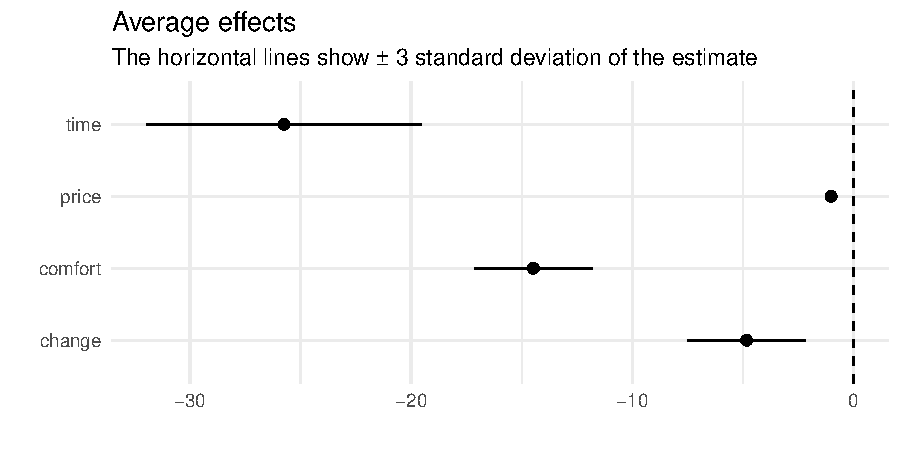
\includegraphics{rprobitb_oelschlaeger_bauer-coef-model-train}

The results indicate that the deciders value one hour travel time by about 26 euros, an additional change by 5 euros, and a more comfortable class by 15 euros.\footnote{We note that these results are consistent with the ones that are presented in a vignette of \pkg{mlogit} entitled "The random parameters (or mixed) logit model" on the same data set but using the logit model.} Calling the \fct{summary} method on the estimated \class{RprobitB\_fit} object yields additional information about the (transformed) Gibbs samples. The method receives a list \code{FUN} of arbitrary functions that can compute point estimates of the Gibbs samples, per default \fct{mean} for the arithmetic mean, \fct{stats::sd} for the standard deviation, and \fct{R\_hat} for the Gelman-Rubin statistic \citep{Gelman:1992}\footnote{A Gelman-Rubin statistic (a lot) greater than 1 indicates convergence issues of the Gibbs sampler.}:

\begin{Schunk}
\begin{Sinput}
> FUN <- c("mean" = mean, "sd" = stats::sd, "R^" = RprobitB::R_hat)
> summary(model_train, FUN = FUN)
\end{Sinput}
\begin{Soutput}
Probit model
Formula: choice ~ price + time + comfort + change | 0 
R: 1000, B: 500, Q: 1

Utility normalization
Level: Utility differences with respect to alternative 'B'.
Scale: Coefficient of effect 'price' (alpha_1) fixed to -1.

Gibbs sample statistics
          mean      sd      R^
 alpha
                              
     1   -1.00    0.00    1.00
     2  -25.95    2.08    1.00
     3  -14.52    0.84    1.00
     4   -4.96    0.87    1.03

 Sigma
                              
   1,1  660.03   58.54    1.00
\end{Soutput}
\end{Schunk}

Calling the \fct{plot} method with the additional argument \code{type = "trace"} plots the trace of the transformed and thinned Gibbs samples after the burn-in:

\begin{Schunk}
\begin{Sinput}
> par(mfrow = c(1,2))
> plot(model_train, type = "trace")
\end{Sinput}
\end{Schunk}
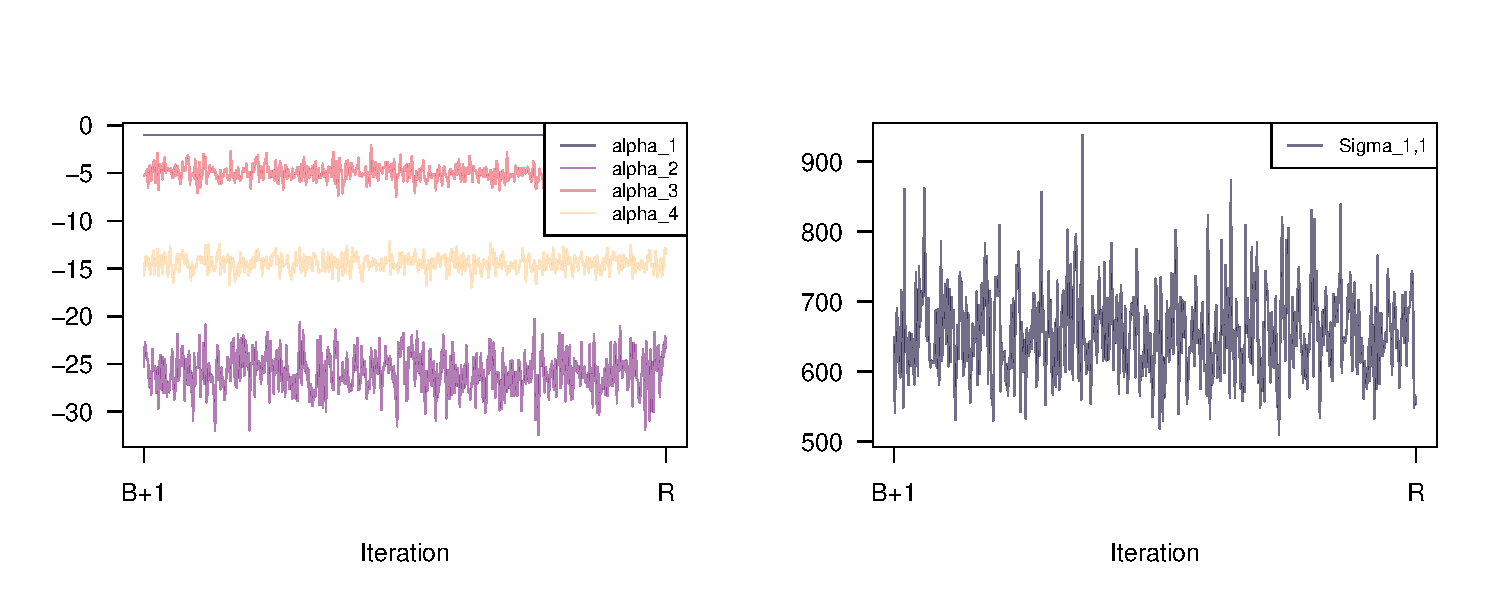
\includegraphics{rprobitb_oelschlaeger_bauer-model-train-trace}

Additionally, we can visualize the autocorrelation of the Gibbs samples via the argument \code{type = "acf"}, below exemplary for \code{alpha\_4} and \code{Sigma\_1,1}). The boxes in the plot's top-right corner state the total sample size TSS, given by (\code{R} - \code{B}) / \code{Q}, the effective sample size ESS, and the factor by which TSS is larger than ESS. The effective sample size is the value $\text{TSS} / (1 + 2\sum_{k\geq 1} \rho_k)$, where $\rho_k$ is the $k$-th order autocorrelation of the Gibbs samples \citep{Marin:2014}. The autocorrelations are estimated via the \fct{stats::acf} function.

\begin{Schunk}
\begin{Sinput}
> par(mfrow = c(1,2))
> plot(model_train, type = "acf", ignore = c("alpha_1", "alpha_2", "alpha_3"))
\end{Sinput}
\end{Schunk}
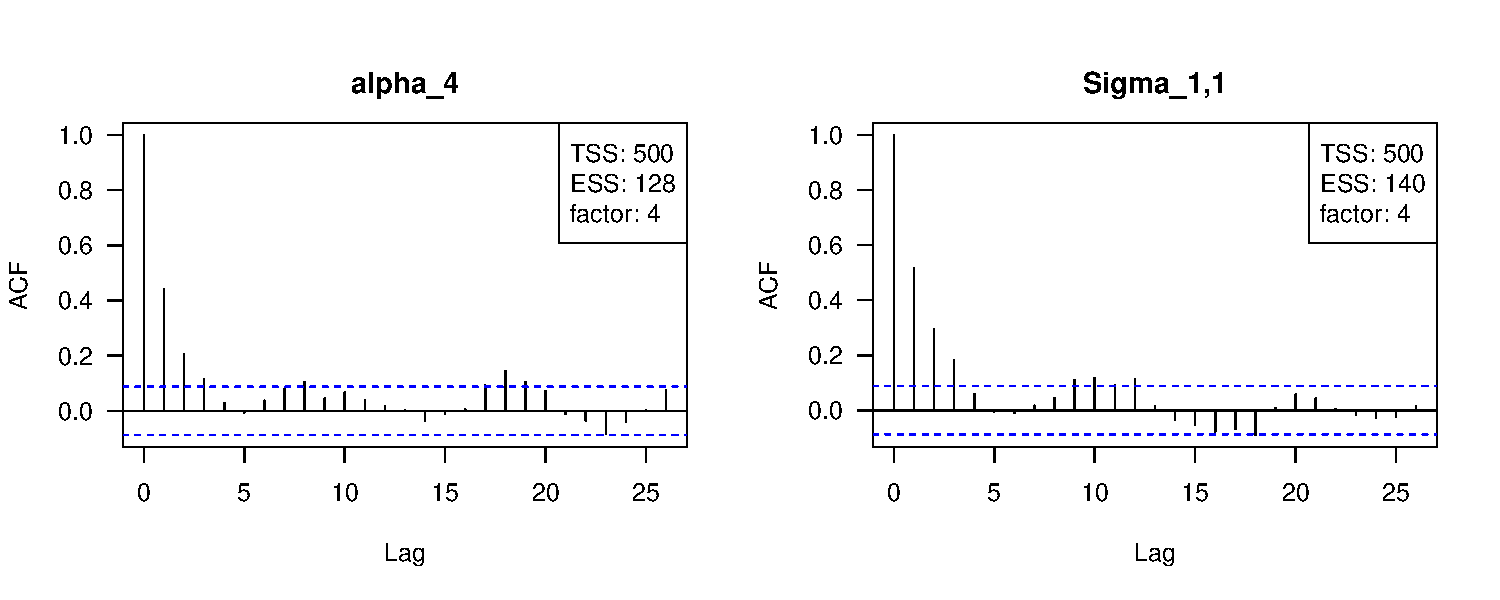
\includegraphics{rprobitb_oelschlaeger_bauer-model-train-acf}

To obtain more independent samples, the \fct{transform} method can be used to increase the thinning factor:\footnote{The function can also be used to increase the length of the burn-in period (via \code{transform(model\_train, B = B\_new)}) or to change the utility scale, for example \code{transform(model\_train, scale = Sigma\_1 ~ 1)}.}

\begin{Schunk}
\begin{Sinput}
> model_train <- transform(model_train, Q = 5)
\end{Sinput}
\end{Schunk}

\subsection{Estimating a joint normal mixing distribution} \label{subsec:normal_mix}

We demonstrate how to estimate a joint normal mixing distribution in \pkg{RprobitB} on the basis of another real-data example. To enable comparison across methods and implementations, we use another data set from \pkg{mlogit}. Their results (using the logit model) are documented in the package vignette entitled "Exercise 3: Mixed logit model".

\paragraph{Example 3: Electricity suppliers.}

The \code{Electricity} data set from \pkg{mlogit} contains choices of residential electricity customers that were asked to decide between four contract offers of hypothetical electricity suppliers. Heterogeneity in choice behavior is expected here, because customers might value certain contract characteristics differently based on their living conditions. In particular, the contract offers differed in 6 characteristics: their fixed price \code{pf} per kilowatt hour, their contract length \code{cf}, whether the supplier is a local company (boolean \code{loc}), whether the supplier is a well known company (boolean \code{wk}), whether the supplier offers a time-of-day electricity price which is higher during the day and lower during the night (boolean \code{tod}), and whether the supplier's price is seasonal dependent (boolean \code{seas}).

The following lines prepare the data set for estimation. We first use the convenience function \fct{as\_cov\_names} that relabels the data columns for alternative specific covariates into the required format \code{"<covariate>\_<alternative>"}:

\begin{Schunk}
\begin{Sinput}
> data("Electricity", package = "mlogit")
> Electricity <- as_cov_names(
+    choice_data = Electricity,
+    cov = c("pf","cl","loc","wk","tod","seas"),
+    alternatives = 1:4
+  )
\end{Sinput}
\end{Schunk}

Via the \code{re = c("cl","loc","wk","tod","seas")} argument, we specify that we want to model random effects for all but the price coefficient, which we again will fix to \code{-1} to interpret the other estimates as monetary values (cf.\ Example 1):

\begin{Schunk}
\begin{Sinput}
> data_elec <- prepare_data(
+    form = choice ~ pf + cl + loc + wk + tod + seas | 0,
+    choice_data = Electricity,
+    re = c("cl","loc","wk","tod","seas")
+  )
> model_elec <- fit_model(data_elec, R = 1000, scale = pf ~ -1)
\end{Sinput}
\end{Schunk}

Calling the \fct{coef} method on the estimated model returns a table of the average effects and the estimated (marginal) variances of the mixing distribution:

\begin{Schunk}
\begin{Sinput}
> coef(model_elec)
\end{Sinput}
\begin{Soutput}
        Estimate   (sd) Variance   (sd)
1   pf     -1.00 (0.00)       NA   (NA)
2   cl     -0.25 (0.03)     0.31 (0.03)
3  loc      2.79 (0.25)     7.43 (1.25)
4   wk      2.07 (0.21)     3.84 (0.67)
5  tod     -9.70 (0.21)    10.72 (1.32)
6 seas     -9.89 (0.18)     6.25 (1.03)
\end{Soutput}
\end{Schunk}

We can for example deduce, that a longer contract length has a negative effect on average (-0.25). However, our model shows that 32\% of the customers still prefer to have a longer contract length. This share is estimated by computing the proportion under the mixing distribution that yields a positive coefficient for \code{cl}:

\begin{Schunk}
\begin{Sinput}
> cl_mu <- coef(model_elec)["cl","mean"]
> cl_sd <- sqrt(coef(model_elec)["cl","var"])
> pnorm(cl_mu / cl_sd)
\end{Sinput}
\begin{Soutput}
[1] 0.3249726
\end{Soutput}
\end{Schunk}

The estimated joint mixing distribution additionally allows to infer correlations between effects. They can be extracted via the \fct{cov\_mix} function (setting \code{cor = FALSE} would return the covariances). For example, we see a correlation of 0.79 between \code{loc} and \code{wk} (deciders that prefer local suppliers also prefer well known companies):

\begin{Schunk}
\begin{Sinput}
> round(cov_mix(model_elec, cor = TRUE), 2)
\end{Sinput}
\begin{Soutput}
        cl  loc   wk   tod  seas
cl    1.00 0.09 0.07 -0.04 -0.10
loc   0.09 1.00 0.79  0.13  0.04
wk    0.07 0.79 1.00  0.14  0.03
tod  -0.04 0.13 0.14  1.00  0.55
seas -0.10 0.04 0.03  0.55  1.00
\end{Soutput}
\end{Schunk}

\subsection{Estimating a latent class model} \label{subsec:latent_classes}

\pkg{RprobitB} allows to specify a Gaussian mixture as the mixing distribution (cf.\ Section \ref{subsec:heterogeneity}), which allows for (a) a flexible approximation of the true underlying mixing distribution and (b) a preference based classification of the deciders. To estimate such a latent mixture, pass the list \code{latent\_classes = list("C" = C)} to \fct{fit\_model}, with \code{C} being the number (greater or equal 1) of latent classes (set to 1 per default). We here assume that $C$ is known and fixed. The following Sections \ref{subsec:weight_update} and \ref{subsec:dp_update} present two updating schemes in which $C$ does not need to be pre-specified.

\paragraph{Example 2: Simulated choices (cont.).}

We previously simulated the \class{RprobitB\_data} object \code{data\_sim} from a probit model with two latent classes. We now aim to reproduce the model parameters from the data generating process:

\begin{Schunk}
\begin{Sinput}
> model_sim <- fit_model(
+    data = data_sim, R = 1000, latent_classes = list("C" = 2), seed = 1
+  )
> summary(model_sim)
\end{Sinput}
\begin{Soutput}
Probit model
Formula: choice ~ var1 | var2 | var3 
R: 1000, B: 500, Q: 1

Utility normalization
Level: Utility differences with respect to alternative 'alt2'.
Scale: Coefficient of the 1. error term variance fixed to 1.

Latent classes
C = 2 

Gibbs sample statistics
          true    mean      sd      R^
 alpha
                                      
     1   -1.00   -0.99    0.09    1.20
     2    0.00   -0.03    0.04    1.03
     3    1.00    0.93    0.09    1.07

 s
                                      
     1    0.70    0.70    0.09    1.01
     2    0.30    0.30    0.09    1.01

 b
                                      
   1.1    2.00    2.04    0.21    1.06
   1.2   -0.50   -0.51    0.28    1.00
   2.1    1.00    0.74    0.41    1.05
   2.2    1.00    1.20    0.32    1.00

 Omega
                                      
 1.1,1    0.31    0.23    0.14    1.71
 1.1,2    0.71    0.37    0.25    1.52
 1.2,2    4.67    4.33    1.16    1.04
 2.1,1    1.67    1.18    0.51    1.11
 2.1,2   -1.20   -0.71    0.35    1.03
 2.2,2    0.87    0.66    0.31    1.01

 Sigma
                                      
   1,1    1.00    1.00    0.00    1.00
\end{Soutput}
\end{Schunk}

Comparing the columns of true parameters (\code{true}) and Gibbs sample means (\code{mean}), we deduce that the model parameters (especially those characterizing the latent classes) can be estimated consistently.

\subsection{Weight-based update of the latent classes} \label{subsec:weight_update}

Adding \code{"weight_update" = TRUE} to the list for the \code{latent\_classes} argument of \fct{fit\_model} executes the following weight-based updating scheme of the latent classes (analogue to \cite{Bauer:2019}):

\begin{itemize}
  \item Class $c$ is removed, if $s_c<\varepsilon_{\text{min}}$, i.e.\ if the class weight $s_c$ drops below some threshold $\varepsilon_{\text{min}}$. This case indicates that class $c$ has a negligible impact on the mixing distribution.
  \item Class $c$ is splitted into two classes $c_1$ and $c_2$, if $s_c>\varepsilon_\text{max}$. This case indicates that class $c$ has a high influence on the mixing distribution whose approximation can potentially be improved by increasing the resolution in directions of high variance. Therefore, the class means $b_{c_1}$ and $b_{c_2}$ of the new classes $c_1$ and $c_2$ are shifted in opposite directions from the class mean $b_c$ of the old class $c$ in the direction of the highest variance.
  \item Classes $c_1$ and $c_2$ are joined to one class $c$, if $\lVert b_{c_1} - b_{c_2} \rVert<\varepsilon_{\text{distmin}}$, i.e.\ if the euclidean distance between the class means $b_{c_1}$ and $b_{c_2}$  drops below some threshold $\varepsilon_{\text{distmin}}$. This case indicates location redundancy which should be repealed. The parameters of $c$ are assigned by adding the values of $s$ from $c_1$ and $c_2$ and averaging the values for $b$ and $\Omega$.
\end{itemize}

The values for $\varepsilon_{\text{min}}$, $\varepsilon_{\text{max}}$ and $\varepsilon_{\text{distmin}}$ can be specified via the \code{latent\_classes} argument (per default \code{epsmin = 0.01}, \code{epsmax = 0.99}, and \code{distmin = 0.1}).

\paragraph{Example 2: Simulated choices (cont.).}

For our simulation example, we additionally specify \code{"C" = 10} (the initial number of latent classes) and \code{"buffer" = 5} (to execute the updating scheme only in every $buffer$-th iteration):

\begin{Schunk}
\begin{Sinput}
> model_sim <- fit_model(
+    data = data_sim, R = 1000, seed = 1,
+    latent_classes = list("C" = 10, "weight_update" = TRUE, "buffer" = 5),
+  )
\end{Sinput}
\end{Schunk}

The updating behavior of the class numbers can be visualized as follows:

\begin{Schunk}
\begin{Sinput}
> plot(model_sim, type = "class_seq")
\end{Sinput}
\end{Schunk}
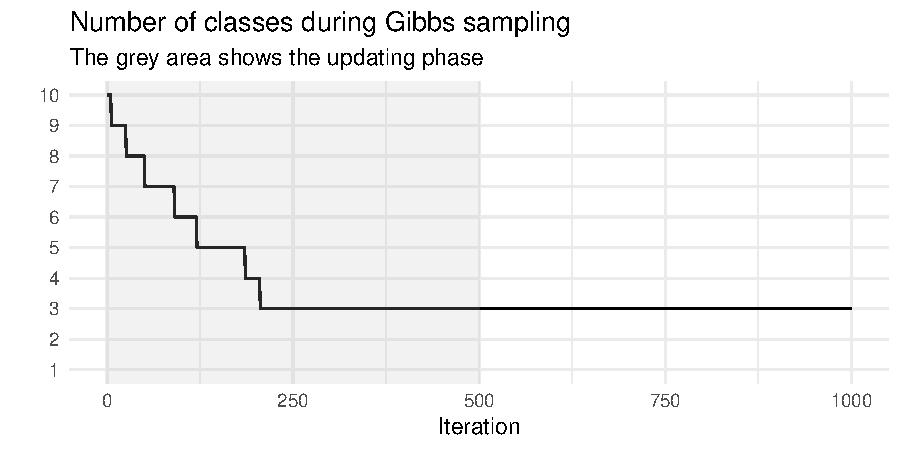
\includegraphics{rprobitb_oelschlaeger_bauer-model-sim-class-seq}

\subsection{Dirichlet process-based update of the latent classes} \label{subsec:dp_update}

The Dirichlet process is a Bayesian nonparametric method that adds as many mixture components to the mixing distribution as needed for a good approximation. We briefly formulate the theory and refer to \cite{Neal:2000} for more details.

A priori, the mixture weights $(s_c)_c$ are given a Dirichlet prior with concentration parameter $\delta/C$. For the class allocation variables $z$, \cite{Rasmussen:2000} shows that
\begin{align}
  \label{eq:all_prob}
  \Pr(z \mid \delta) = \frac{\Gamma(\delta)}{\Gamma(N+\delta)} \prod_{c=1}^C \frac{\Gamma(m_c + \delta/C)}{\Gamma(\delta/C)},
\end{align}
where $\Gamma(\cdot)$ denotes the gamma function and $m_c$ the size of class $c$. Crucially, equation \eqref{eq:all_prob} is independent of the class weights $(s_c)_c$ (in contrast to the conditional posterior distribution stated in Section \ref{subsec:prior_and_posterior}). From this equation, \cite{Li:2019} shows that
\begin{align*}
  \Pr(z_n = c \mid z_{-n}, \delta) = \frac{m_{c,-n} + \delta/C}{N-1+\delta} \to \frac{m_{c,-n}}{N-1+\delta},
\end{align*}
where the limit is taken as $C$ approaches infinity, and $z_{-n}$ denotes the vector $z$ without the $n$-th element. Now,
\begin{align*}
  1 - \sum_{c = 1}^C \frac{m_{c,-n}}{N-1+\delta} = \frac{\delta}{N-1+\delta}
\end{align*}
equals the probability that a new cluster for observation $n$ is created. This probability is directly proportional to the prior parameter $\delta$ \citep{Neal:2000}: a greater value for $\delta$ encourages the creation of new clusters, smaller values increase the probability of an allocation to an already existing class. The number of clusters can theoretically rise to infinity, however, as we delete unoccupied clusters, $C$ is bounded by $N$.

The Dirichlet process directly integrates into our existing Gibbs sampler: given $(\beta_n)_n$, we update the class means $b_c$ and covariance matrices $\Omega_c$ by means of their posterior predictive distribution. The mean vector and covariance matrix for new generated clusters are drawn from their prior predictive distribution (\cite{Li:2019} provides the formulas). The full updating scheme is implemented in the function \fct{update\_classes\_dp} and can be executed within the estimation routine \fct{fit\_model} by adding \code{dp\_update = TRUE} to the list argument for \code{latent\_classes}.

\paragraph{Example 4: Online chess strategy.}

We demonstrate the Dirichlet process updating scheme via an example from online chess. \pkg{RprobitB} containes revealed gambling preference data of chess players in the yearly bullet arena 2022 on the online chess platform https://lichess.org: at the beginning of each game, both players can choose to trade half of their clock time\footnote{Both players start a game with a time credit of one minute, which is consumend when it's their turn to make a move. A player whos time runs up looses the game automatically.} against the option to win an extra tournament point in case they win the game. The tournament lasted 4 hours, participants were paired again immediately after they finished a game, and the player with the most tournament points in the end won the event. The platform calls the trade clock time against a potential extra tournament "berserking". Several questions regarding the trade "clock time against a potential extra tournament" (which the platform calls "berserking") immediately arise: Do higher-rated chess players prefer to gamble? Does the remaining tournament time have an influence on the berserking choice? Can players be classified based on their revealed preferences to berserk?

The \code{choice\_berserk} data set provides the following information: whether a player berserked (\code{berserk = 1} if yes), wether they had the \code{white} pieces, their \code{rating} (a value provided by the platform indicating the playing strength), the rating difference \code{rating\_diff} to the opponent, whether they lost the game (\code{lost = 1} if yes), the remaining tournament time \code{min\_rem} in minutes, and whether they are currently on a winning \code{streak} (which gives extra points). We additionally consider the lagged covariates \code{berserk.1} (the berserking choice in the previous game) and \code{lost.1} (the result of a player's previous game), which can be created via the convenience function \fct{choice\_berserk}. We specify random effects for the rating difference and the result of the previous game, aiming to classify the chess players based on their berserking choice to these circumstances.

\begin{Schunk}
\begin{Sinput}
> choice_berserk <- create_lagged_cov(
+    choice_data = RprobitB::choice_berserk,
+    column = c("berserk","lost"), k = 1, id = "player_id"
+  )
> data <- prepare_data(
+    form = berserk ~ 0 | white + rating + rating_diff + min_rem + streak + berserk.1 + lost.1 + 1,
+    re = c("rating_diff","lost.1"), choice_data = choice_berserk, id = "player_id", idc = "game_id",
+    standardize = c("rating","rating_diff","min_rem"), impute = "zero"
+  )
> model_berserk <- fit_model(
+    data, latent_classes = list("dp_update" = TRUE, "C" = 10), R = 5000
+  )
\end{Sinput}
\end{Schunk}

Estimating this model with $N = 6174$ deciders, $T = 1$ to $177$ choice occasions and $126902$ choices in total took about 4 hours computation time. For convenience, we pre-computed the model and saved the resulting \code{model\_berserk} object in the package:

\begin{Schunk}
\begin{Sinput}
> data(model_berserk, package = "RprobitB")
> coef(model_berserk)
\end{Sinput}
\begin{Soutput}
                     Estimate   (sd) Variance   (sd)
1           white_0      0.04 (0.02)       NA   (NA)
2          rating_0      0.11 (0.01)       NA   (NA)
3         min_rem_0     -0.04 (0.01)       NA   (NA)
4          streak_0      0.27 (0.03)       NA   (NA)
5       berserk.1_0     -1.21 (0.02)       NA   (NA)
6             ASC_0      2.05 (0.03)       NA   (NA)
7  rating_diff_0 [1]    -0.10 (0.02)     0.08 (0.01)
8  rating_diff_0 [2]    -0.98 (0.06)     0.25 (0.05)
9  rating_diff_0 [3]    -1.65 (0.21)     1.72 (0.32)
10      lost.1_0 [1]     0.98 (0.09)     0.54 (0.10)
11      lost.1_0 [2]    -0.03 (0.08)     0.28 (0.06)
12      lost.1_0 [3]    -1.09 (0.18)     0.99 (0.21)
\end{Soutput}
\end{Schunk}

The classes can be visualized via calling the \fct{plot} method with the additional argument \code{type = mixture}:

\begin{Schunk}
\begin{Sinput}
> plot(model_berserk, type = "mixture")
\end{Sinput}
\end{Schunk}
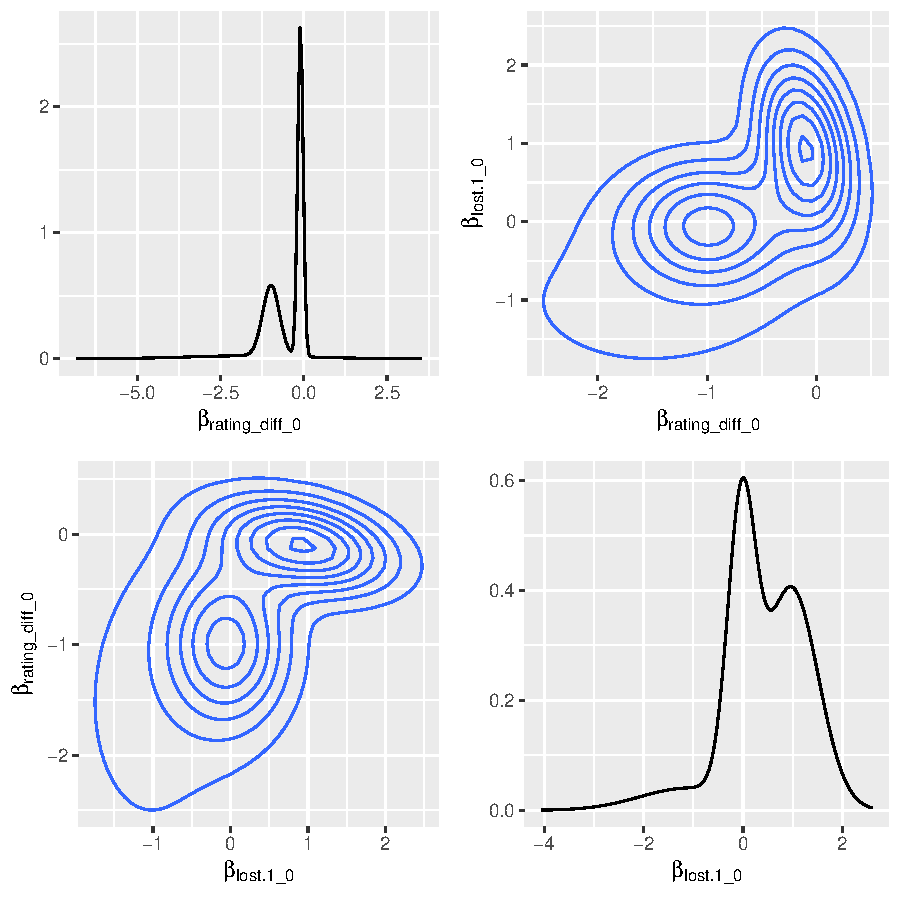
\includegraphics{rprobitb_oelschlaeger_bauer-model-berserk-mixture}

\begin{Schunk}
\begin{Sinput}
> head(preference_classification(model_berserk), n = 5)
\end{Sinput}
\begin{Soutput}
                        1     2     3 est
a_chess_player_123  0.556 0.376 0.068   1
a_nizamoff          0.276 0.648 0.076   2
a_salikhov          0.828 0.172 0.000   1
a137p314            0.616 0.368 0.016   1
a1bharadwaj2019_64k 0.684 0.296 0.020   1
\end{Soutput}
\end{Schunk}

\section{Choice prediction} \label{sec:choice_prediction}

\pkg{RprobitB} provides a \fct{predict} method for in-sample and out-of-sample prediction. The former case refers to reproducing the observed choices on the basis of the covariates and the fitted model and subsequently using the deviations between prediction and reality as an indicator for the model performance. The latter means forecasting choice behavior for changes in the choice attributes. For illustration, we revisit our probit model of travelers deciding between two fictional train route alternatives.

\paragraph{Example 1: Train trips (cont.).}

Per default, the \fct{predict} method returns a confusion matrix, which gives an overview of the in-sample prediction performance: Warning Train p. 69.

\begin{Schunk}
\begin{Sinput}
> predict(model_train)
\end{Sinput}
\begin{Soutput}
    predicted
true    A    B
   A 1034  440
   B  452 1003
\end{Soutput}
\end{Schunk}

By setting the argument \code{overview = FALSE}, the method instead returns predictions on the level of individual choice occasions:\footnote{Incorrect predictions can be analyzed via the convenience function \fct{get\_cov}, which extracts the characteristics of a particular choice situation.}

\begin{Schunk}
\begin{Sinput}
> pred <- predict(model_train, overview = FALSE)
> head(pred, n = 5)
\end{Sinput}
\begin{Soutput}
  id choiceid    A    B true predicted correct
1  1        1 0.92 0.08    A         A    TRUE
2  1        2 0.64 0.36    A         A    TRUE
3  1        3 0.79 0.21    A         A    TRUE
4  1        4 0.18 0.82    B         B    TRUE
5  1        5 0.55 0.45    B         A   FALSE
\end{Soutput}
\end{Schunk}

Apart from the prediction accuracy, the model performance can be evaluated more nuanced in terms of sensitivity and specificity, for example via a receiver operating characteristic (ROC) curve \citep{Fawcett:2006}, using the \pkg{plotROC} package \citep{Sachs:2017}:

\begin{Schunk}
\begin{Sinput}
> library(plotROC)
> ggplot(data = pred, aes(m = A, d = ifelse(true == "A", 1, 0))) +
+    geom_roc(n.cuts = 20, labels = FALSE) +
+    style_roc(theme = theme_grey)
\end{Sinput}
\end{Schunk}
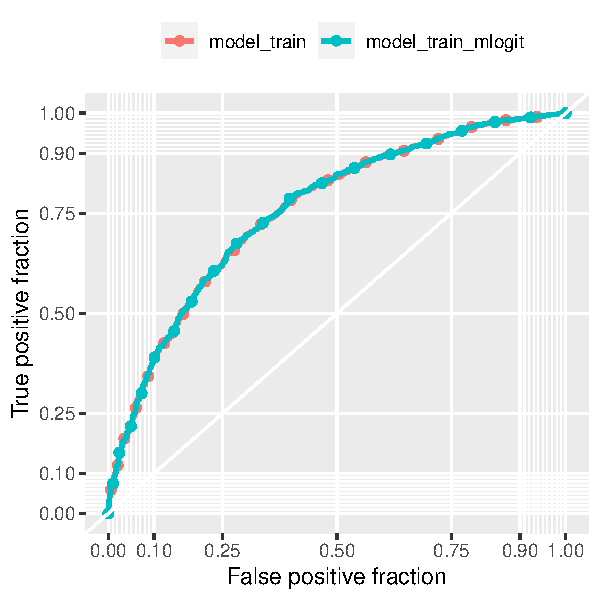
\includegraphics{rprobitb_oelschlaeger_bauer-roc-example}

The \fct{predict} method has an additional \code{data} argument. Per default, \code{data = NULL}, which results into the in-sample case outlined above. Alternatively, \code{data} can be either an \class{RprobitB\_data} object (for example a test subsample extracted via the \fct{train\_test} function) or a data frame of custom choice characteristics.

We demonstrate the second case in the following. Assume that a train company wants to anticipate the effect of a price increase on their market share. By our model, increasing the ticket price from 100 euros to 110 euros (ceteris paribus) draws 15\% of the customers to the competitor who does not increase their prices:

\begin{Schunk}
\begin{Sinput}
> predict(
+    model_train,
+    data = data.frame("price_A" = c(100,110),
+                      "price_B" = c(100,100)),
+    overview = FALSE)
\end{Sinput}
\begin{Soutput}
  id choiceid    A    B prediction
1  1        1 0.50 0.50          A
2  2        1 0.35 0.65          B
\end{Soutput}
\end{Schunk}

However, offering a better comfort class compensates for the higher price and even results in a gain of 7\% market share:

\begin{Schunk}
\begin{Sinput}
> predict(
+    model_train,
+    data = data.frame("price_A" = c(100,110), "comfort_A" = c(1,0),
+                      "price_B" = c(100,100), "comfort_B" = c(1,1)),
+    overview = FALSE)
\end{Sinput}
\begin{Soutput}
  id choiceid    A    B prediction
1  1        1 0.50 0.50          A
2  2        1 0.57 0.43          A
\end{Soutput}
\end{Schunk}

\section{Model selection} \label{sec:model_selection}

\pkg{RprobitB} provides several tools to identify the most appropriate model among competing one, including the information criteria AIC \citep{Akaike:1974}, BIC \citep{Schwarz:1978}, WAIC \citep{Watanabe:2010}, and the Bayes factor.

The WAIC is a Bayesian version of AIC and BIC and defined as $-2 \cdot \text{lppd} + 2\cdot p_\text{WAIC}$, where $\text{lppd} = \sum_i \log \left( S^{-1} \sum_s p_{si} \right)$ is the log-pointwise predictive density, $p_\text{WAIC} = \sum_i \mathbb{V}_{\theta} \log (p_{si})$ is a penalty term proportional to the variance in the posterior distribution, and $p_{si} = \Pr(y_i\mid \theta_s)$ be the probability of choice $y_i$ given the $s$-th set $\theta_s$ of parameter samples from the posterior \citep[p.\ 220]{McElreath:2016}. The $\text{WAIC}$ has a standard error of $\sqrt{n \cdot \mathbb{V}_i \left[-2 \left(\text{lppd} - \mathbb{V}_{\theta} \log (p_{si}) \right)\right]},$ where $n$ is the total number of choices. Both WAIC value and its standard error can be computed via the \fct{WAIC} method.

The Bayes factor is an index of relative posterior model plausibility of one model over another \citep{Marin:2014}: given data $y$ and two models $M_1$ and $M_2$, it is defined as
\begin{align*}
BF(M_1,M_2) = \frac{\Pr(M_1 \mid y)}{\Pr(M_2 \mid y)} = \frac{\Pr(y \mid M_1 )}{\Pr(y \mid M_2)}~/~\frac{\Pr(M_1)}{\Pr(M_2)},
\end{align*}
where per default $\Pr(M_1) = \Pr(M_2) = 0.5$. The value $\Pr(y \mid M)$ denotes the marginal model likelihood, which has no closed form and must be approximated numerically. \pkg{RprobitB} uses the posterior Gibbs samples derived from the \fct{fit\_model} function to approximate the likelihood via the posterior harmonic mean estimator \citep{Newton:1994} in combination with the prior arithmetic mean estimator \citep{Hammersley:1964}. Both estimators converge with rising posterior samples to the marginal model likelihood by the law of large numbers. Convergence is fast if the prior and posterior distribution have a similar shape and strong overlap \citep{Gronau:2017}. The estimators are implemented in the function \code{mml}. \pkg{RprobitB} provides plotting methods for analyzing the convergence behavior, see \code{help(mml, package = "RprobitB")} for details.

\paragraph{Example 1: Train trips (cont.).}

We revisit the probit model of travelers deciding between two fictional train route alternatives. As a competing model to \code{model\_train}, we consider explaining the choices only by the alternative's price, i.e.\ the probit model with the formula \code{choice ~ price | 0`}. The \fct{nested\_model} function helps in estimating such a nested model:

\begin{Schunk}
\begin{Sinput}
> model_train_sparse <- nested_model(model_train, form = choice ~ price | 0)
\end{Sinput}
\end{Schunk}

\pkg{RprobitB} provides the convenience function \fct{model\_selection}, which takes an arbitrary number of \class{RprobitB\_fit} objects and returns a matrix of model selection criteria. The \code{criteria} input is a vector of \code{"npar"} (for the number of model parameters), \code{"LL"} (for the model's log-likelihood value, computed with the point estimates obtained from the Gibbs sample means), \code{"AIC"}, \code{"BIC"}, \code{"WAIC"}, \code{"MMLL"} (the marginal model log-likelihood), \code{"BF"} (for the Bayes factor), and \code{"pred_acc"} (the prediction accuracy). In order to compute WAIC, the marginal model likelihood, and the Bayes factor, the probabilities $p_{si} = \Pr(y_i\mid \theta_s)$ must be pre-computed via the \fct{compute\_p\_si} function:

\begin{Schunk}
\begin{Sinput}
> model_train <- compute_p_si(model_train)
> model_train_sparse <- compute_p_si(model_train_sparse)
> model_selection(
+    model_train, model_train_sparse,
+    criteria = c("npar", "LL", "AIC", "BIC", "WAIC", "MMLL", "BF", "pred_acc")
+  )
\end{Sinput}
\begin{Soutput}
                         model_train model_train_sparse
npar                               4                  1
LL                          -1727.72           -1865.86
AIC                          3463.45            3733.73
BIC                          3487.38            3739.71
WAIC                         3462.95            3734.29
se(WAIC)                        0.16               0.08
pWAIC                           3.93               1.35
MMLL                        -1730.71           -1866.89
BF(*,model_train)                  1             < 0.01
BF(*,model_train_sparse)       > 100                  1
pred_acc                      69.55%             63.40%
\end{Soutput}
\end{Schunk}

\section{Conclusion} \label{sec:conclusion}

% %% The problem
% This paper addressed the problem of specifying mixing distributions in the multinomial probit model with a panel data setting, constituting an important part of the model selection for which the literature does not provide much guidance so far. In the absence of alternatives, many applications of the mixed multinomial probit model rely on different types of standard parametric distributions for modelling heterogeneity in preferences in combination with a likelihood-value based model selection. This course of action is very restrictive and imposes strong assumptions on the distribution of the model parameters that could potentially lead to misspecification and biased estimates.
%
% %% Our solution
% We proposed a new approach that improves the current specification strategies in several ways: First, our approach does not require any distributional assumption, since the latent class setting is flexible enough to approximate practically any distribution shape and allowing for any correlation pattern. Second, the weight-based updating scheme ensures that the number of latent classes does not need to be prespecified. Third, the imposed Bayesian estimation framework avoids many numerical problems that occur in the frequentist approach. Most notably, no likelihood function has to be evaluated nor approximated. Comparing the numerical estimation speed to the non-parametric frequentist approach of \cite{Bauer:2019}, we found that our implementation of the Bayesian approach is at least 10 times faster. The improvement becomes more distinct for panel data settings with a high number of choice occasions. This is due to the fact that for given total sample size $NT$ a large $T$ is beneficial for the Bayesian approach as then the number of vectors $\beta_n,~ n = 1,...,N$ is comparatively small, while in the frequentist approach calculating the likelihood becomes more challenging for increasing the number $T$ of choice situations faced by each of the $N$ individuals. On the other hand, the grid based frequentist approach of \cite{Bauer:2019} can potentially achieve a better approximation (especially of point masses) due to the relatively high number of latent classes. However, this approach requires that a suitable grid is set prior to the estimation with a specification of upper bounds for the coefficients. Additionally, the curse of dimensionality plays a crucial role, which is less of a burden in the Bayesian approach. Note that for a fully specified parametric structure these concerns do not play such a big role also for the frequentist approach.

\section*{Computational details}

The results in this paper were obtained using
\proglang{R}~4.1.3 with the
\pkg{RprobitB}~1.0.0.9000 package. \proglang{R} itself
and all packages used are available from the Comprehensive
\proglang{R} Archive Network (CRAN) at \url{https://CRAN.R-project.org/}.


\section*{Acknowledgments}

This work has been financed partly by the Deutsche Forschungsgemeinschaft (DFG, German Research Foundation) - Projektnummer 356500581 which is gratefully acknowledged.

\bibliography{ref}


\end{document}
